\chapter{Điều khiển và sao chép dữ liệu với Raspberry Pi}
%Có một cách có thể dùng để điều khiển Raspberry Pi
\section{Điều khiển bằng cách kết nối trực tiếp với màn hình, bàn phím và chuột}
\begin{itemize}
\item \textit{Điều khiển}: Kết nối chuột và bàn phím qua các cổng USB. Với màn hình thông thường có 2 loại: màn hình hỗ trợ cổng HDMI và màn hình hổ trợ cổng VGA.
\item \textit{Sao chép dữ liệu}: Sử dụng USB.
\end{itemize}
\subsection{Màn hình hổ trợ cổng HDMI}
Ta kết nối màn hình qua cable HDMI. Có thể bạn sẽ cần tùy chỉnh một số thông sau cho phù hợp:
\subsection{Màn hình hổ trợ cổng VGA}
Để hiển thị được, ta cần có cable chuyển đồi từ VGA sang HDMI.
\begin{figure}[!h]
\begin{center}
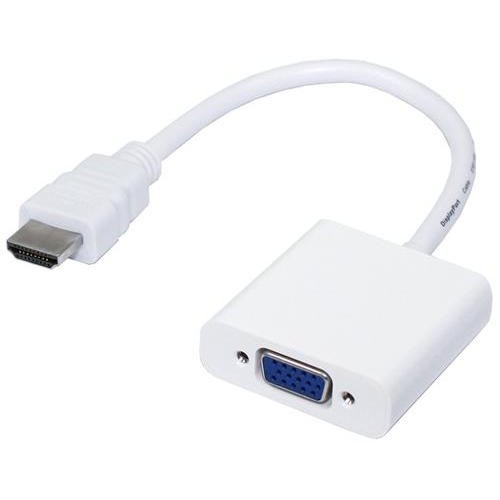
\includegraphics[scale=.3]{remote/images/HDMI-VGA-white}
\end{center}
\caption{Cáp chuyển đổi từ cổng HDMI sang cổng VGA}
\end{figure}
\section{Điều khiển bằng giao tiếp nối tiếp thông qua cổng RS232} \label{Subsec:rs232}
Khi kết nối bằng module RS232, cần cấp nguồn cho Pi hoạt động.
\begin{figure}[!h]
\begin{center}
\subfloat[Module RS232 to TTL]
  {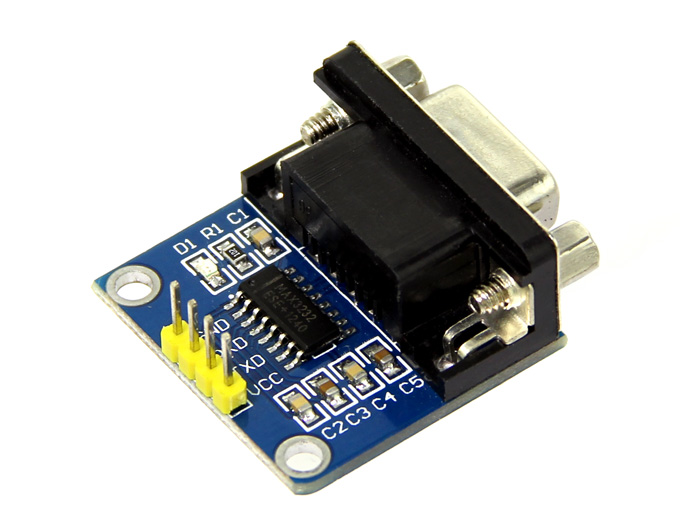
\includegraphics[width=.3\linewidth]{remote/images/RS232-to-ttl}}\hspace{1cm}
\subfloat[Cáp USB to COM]
  {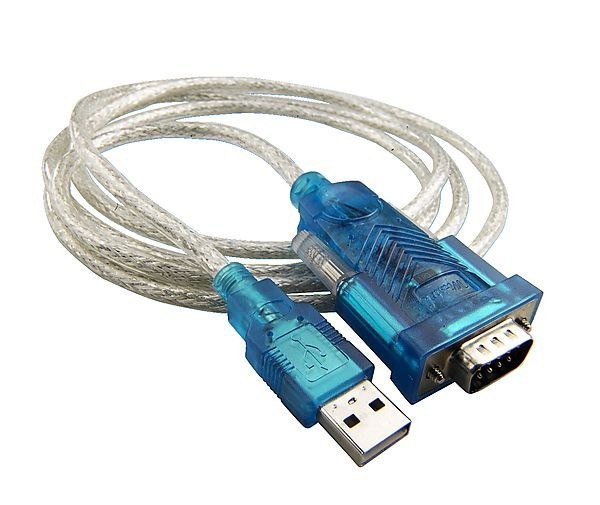
\includegraphics[width=.3\linewidth]{remote/images/cap-usb-to-com}}
\end{center}
\caption{Module RS232 to TTL và Cáp USB to COM}
\end{figure}
\subsection{Cách kết nối}
Thực hiện kết nối Pi và module RS232 như sau:
\begin{center}
\begin{tabular}{c|c}
Pi & RS232\\ \hline
3.3V & VCC\\
TX & TX \\ 
RX & RX\\
GND & GND
\end{tabular}
\end{center}
\subsection{Hệ điều hành Windows}
\begin{itemize}
\item Cài đặt Driver cho cáp, địa chỉ tải về:

\begin{footnotesize}
\verb|https://drive.google.com/file/d/0B6_x_4VdySxqVUJVVVlTTXZfaEE/view?usp=sharing|
\end{footnotesize}
\item Phần mềm Putty, địa chỉ tải về:

\begin{footnotesize}
\verb|http://www.chiark.greenend.org.uk/~sgtatham/putty/download.html|
\end{footnotesize}
\item Cài đặt các phần mềm trên.
\item Kết nối cáp với máy tính, kiểm tra xem cổng COM mấy, để sử dụng giao tiếp: Vào \verb|Device Manager|, để kiểm tra như hình \ref{Fig:COM7}.
\begin{figure}[!h]
\begin{center}
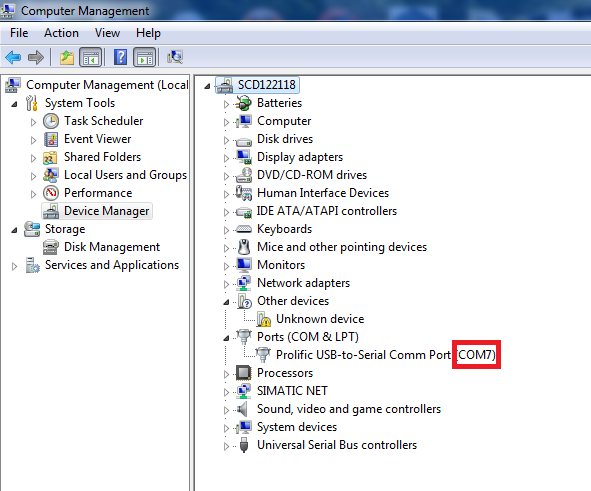
\includegraphics[scale=.5]{remote/images/COM7-Putty}
\end{center}
\caption{Địa chỉ COM của cáp trên máy tính}\label{Fig:COM7}
\end{figure}
\newpage
\item Mở chương trình Putty lên để kết nối: Chọn \verb|Serial| và tên cổng \verb|COM| trong ô \verb|Serial line|, tốc độ truyền trong ô \verb|Speed| là \verb|115200|, như hình \ref{Fig:Putty}.
\begin{figure}[!h]
\begin{center}
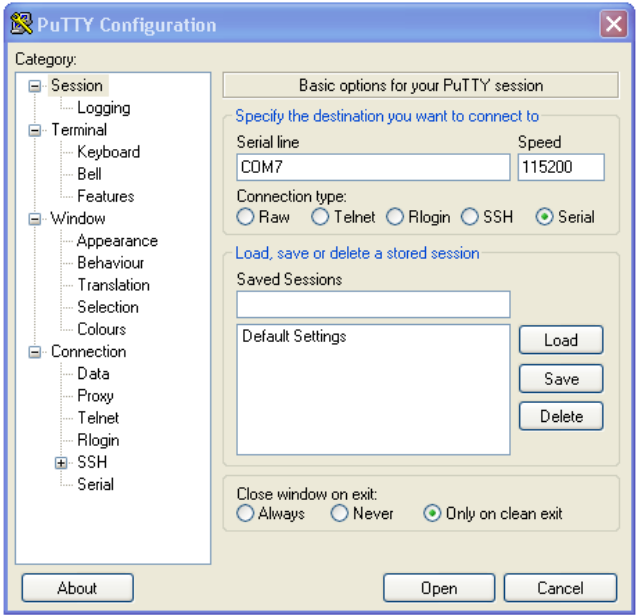
\includegraphics[scale=.4]{remote/images/Putty}
\end{center}
\caption{Thiết lập các thông số cho Putty để kết nối}\label{Fig:Putty}
\end{figure}
\item Nhấn \verb|Open|, vào màn hình đen, Enter thêm một lần nữa.
\item Nhập username và password để đăng nhập.
\end{itemize}
\subsection{Hệ điều hành Ubuntu}
\begin{itemize}
\item Cài đặt gói phần mềm \verb|screen|: \verb|sudo apt-get install screen| trên máy tính Ubuntu.
\item Chạy lệnh sau: \verb|sudo screen /dev/ttyUSB0 115200|
\item Thực hiện xong lệnh trên, ta nhấn Enter một lần nữa để kết nối với Pi.
\item Nhập username và password để đăng nhập.
\item Sao chép dữ liệu: dùng USB.
%\item[$\ast$] Ta có thể dùng Putty (trên hệ điều hành Window) để điều khiển: chọn \verb|Serial|, điền vào khung \verb|Serial line| tên cổng (ví dụ: COM1, COM2,\ldots), trong khung \verb|Speed| điền tốc độ là \verb|115200|. Nhập username và password để đăng nhập.
\end{itemize}
\section{Điều khiển bằng giao tiếp nối tiếp thông qua cáp USB to COM PL2303}
Khi kết nối bằng cáp USB to COM PL2303 thì không cần cấp nguồn ngoài cho Pi hoạt động (do Pi sẽ lấy nguồn từ cổng USB thông qua cáp).
\begin{figure}[!h]
\begin{center}
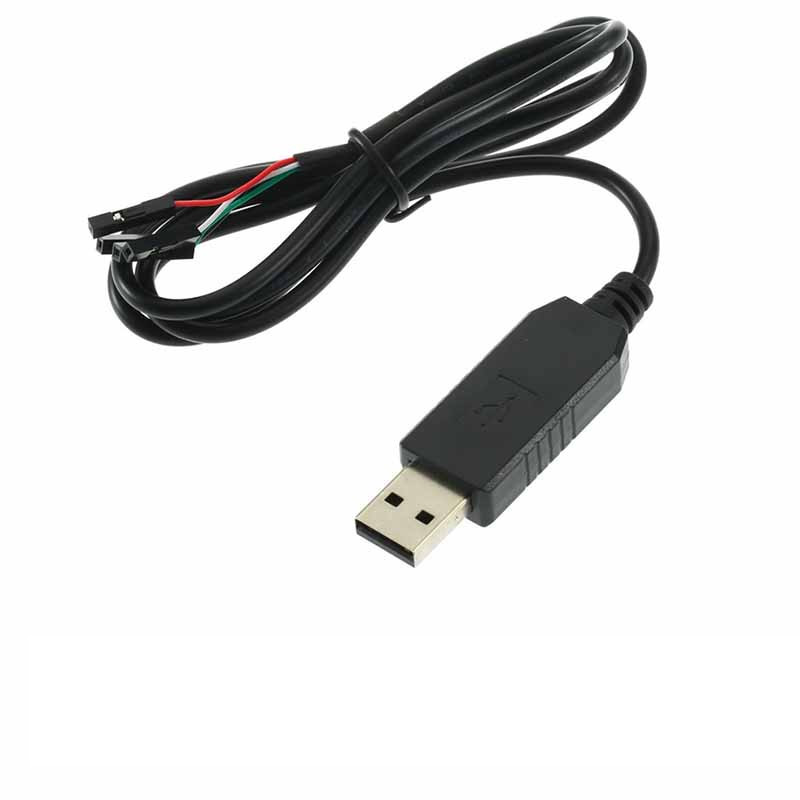
\includegraphics[scale=.3]{remote/images/cap-usb-to-com-pl2303}
\end{center}
\caption{Cáp USB to COM PL2303}
\end{figure}
\begin{itemize}
\item Thực hiện kết nối Pi và cáp USB to COM PL2303 như sau:
\begin{center}
\begin{tabular}{c|c|c}
Pi & PL2303 & Màu dây\\ \hline
5V & VCC & Đỏ\\
TX & RX & Trắng\\ 
RX & TX & Xanh\\
GND & GND & Đen
\end{tabular}
\end{center}
\item Phần cài đặt và điều khiển tương tự như cổng RS232 (xem \textit{mục \ref{Subsec:rs232} trang \pageref{Subsec:rs232}}).
\item Khi sử dụng cáp PL2303 ta sử dụng Driver khác mới kết nối được, địa chỉ tải về:

\begin{footnotesize}
\verb|http://www.prolific.com.tw/US/ShowProduct.aspx?p_id=225&pcid=41|
\end{footnotesize}
\item Giải nén file \verb|PL2303_Prolific_DriverInstaller_v1_12_0.zip| vừa tải về và chạy file \verb|PL2303_Prolific_DriverInstaller_v1.7.0.exe| để cài đặt.
\item Phần còn lại thực hiện giống như mục \ref{Subsec:rs232} trên cả hệ điều hành Windows và hệ điều hành Ubuntu.
\end{itemize}
\section{Điều khiển từ xa khi Raspberry Pi có kết nối mạng}
Khi Raspberry Pi có kết nối mạng Internet, ta có thể dùng các phần mềm: \verb|SSH|, \verb|Remote Desktop|, \verb|VNC|,\ldots~ để điều khiển.
\begin{itemize}
\item Kiểm tra địa chỉ IP của Pi bằng phần mềm: ipscan (trên Windows) hoặc nmap (trên Ubuntu).
\begin{itemize}
\item Phần mềm \verb|ipscan|: giao diện trực quan, dễ sử dụng.
\item Chương trình \verb|nmap| trên Ubuntu:
\begin{list}{+}{}
\item Cài đặt chương trình:
\begin{lstlisting}[language=bash]
sudo apt-get install nmap
\end{lstlisting}
\item Tìm các địa chỉ IP trong mạng nội bộ:
\begin{lstlisting}[language=bash]
sudo nmap -sP 192.168.1.1-254
\end{lstlisting}
THay đổi địa chỉ IP \verb|192.168.1.1| cho phụ hợp với địa chỉ IP của bạn.
\end{list}
\end{itemize}
\item Chọn chương trình phù hợp để điều khiển Raspberry Pi: 
\begin{itemize}
\item Với \verb|SSH|: không hổ trợ giao diện đồ họa.
\begin{lstlisting}[language=bash]
ssh pi@192.168.0.100
\end{lstlisting}
Trong đó: \verb|pi| là tên user bạn cần đăng nhập, kế tiếp là địa chỉ IP của Raspberry Pi.
\item Với \verb|VNC| hoặc \verb|Remote Desktop|: có hổ trợ giao diện đồ họa.
\item[$\ast$]  Với \verb|Remote Desktop| Pi cần cài đặt \verb|xrdp|:
\begin{lstlisting}[language=bash]
sudo apt-get install xrdp
\end{lstlisting}
\end{itemize}
\item Tùy theo chương trình bạn chọn: ta cần phải nhập địa chỉ IP, username và password (nếu có yêu cầu điền số \verb|port|: ta điền 22).
\item Sao chép dữ liệu:
\begin{itemize}
\item Trên Window: dùng \verb|Winscp|.
\item Trên Ubuntu: dùng \verb|FileZilla|.
\begin{figure}[!h]
\begin{center}
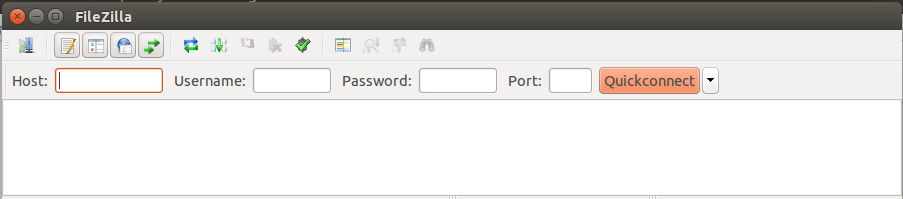
\includegraphics[scale=.45]{remote/images/FileZilla}
\end{center}
\caption{Sao chép dữ liệu từ Raspberry Pi với FileZilla}
\end{figure}
\begin{list}{+}{}
\item \verb|Host|: điền địa chỉ IP.
\item \verb|Username|: tên cần đăng nhập.
\item \verb|Password|: mật khẩu đăng nhập cho tài khoản ở ô \verb|Username|.
\item \verb|Port|: điền số 22.
\end{list}
\item[$\ast$] Ta cũng cần nhập vào thông tin như trên để truy cập được Pi.
\end{itemize}
\item \textit{Lưu ý}: Phần trình bày trên áp ngay cho mạng nội bộ, khi không phải mạng nội bộ ta cần cấu hình mạng rồi mới áp dụng được hướng dẫn ở phần này.
\end{itemize}
\section{Điều khiển Raspberry Pi từ xa với giao diện đồ họa khi có kết nối Internet}
\subsection{Sử dụng VNC trên Window}
\subsection{Sử dụng VNC trên Ubuntu}
\begin{list}{--}{}
\item Cài đặt phần mềm \verb|Remote Desktop Viewer| (trong Ubuntu Software Center).
\item Cài đặt VNC trên Raspberry Pi:
\begin{list}{+}{}
\item Cài đặt \verb|TightVNC Server| trên Pi:
\begin{lstlisting}[language=bash]
$ sudo apt-get install tightvncserver
\end{lstlisting}
\item Cài đặt password để \verb|VNC Client| kết nối với \verb|VNC Server| trên Pi:
\begin{lstlisting}[language=bash]
$ tightvncserver
\end{lstlisting}
Nhập password 2 lần (tối đa 8 ký tự). Và ghi nhớ password này.

Xuất hiện dòng bên dưới:
\begin{lstlisting}[language=bash]
Would you like to enter a view-only password (y/n)?
\end{lstlisting}
Nhấn \verb|n| rồi \verb|Enter|.
\end{list}
\item Sử dụng \verb|VNC| giao tiếp giữa máy tính Ubuntu và Pi:
\begin{list}{+}{}
\item Sử dụng \verb|ssh| kết nối với Pi.
\item Gõ lệnh sau: 
\begin{lstlisting}[language=bash]
$ vncserver :1
\end{lstlisting}
\item Mở phần mềm \verb|Remote Desktop Viewer|, click vào biểu tượng có chữ \verb|Connect| trên thanh công cụ. Xuất hiện hộp thoại như \ref{VNC-1}.
\item Trong ô \verb|Protocol|: chọn \verb|VNC|.  Trong ô \verb|Host| điền vào địa chỉ IP kèm với số \verb|:1|, ví dụ: \verb|192.168.0.102:1|, như hình \ref{VNC-2}.
\begin{figure}[!h]
\begin{center}
	\subfloat[Mở phần mềm \textsf{Remote Desktop Viewer}\label{VNC-1}]
	{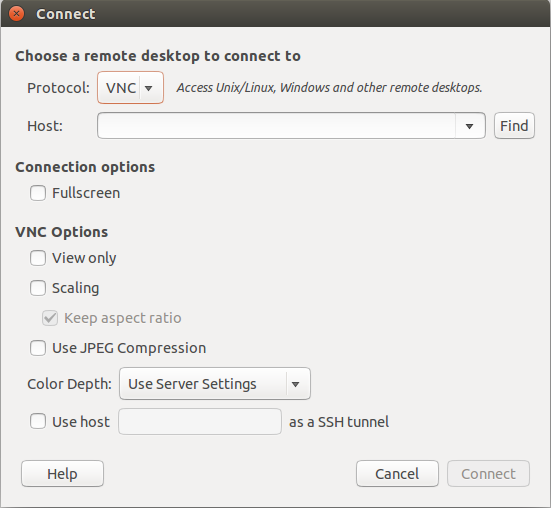
\includegraphics[scale=.35]{remote/images/VNC-1}} \hspace{1cm}
	\subfloat[Điền thông tin để kết nối qua \textsf{VNC}\label{VNC-2}]
	{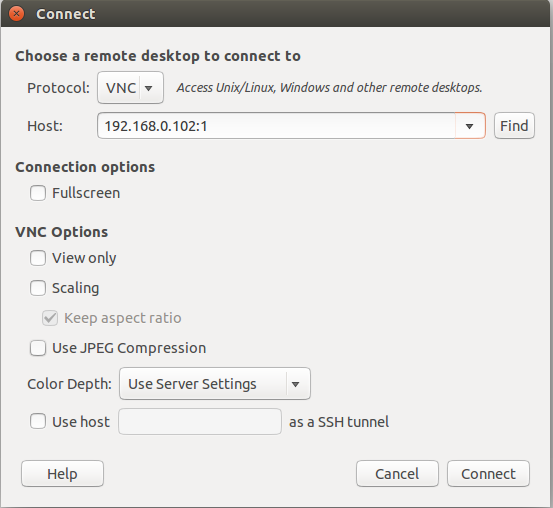
\includegraphics[scale=.35]{remote/images/VNC-2}}
\end{center}
\caption{Sử dụng \textsf{Remote Desktop Viewer}}
\end{figure}
\item Nhấn vào \verb|Connect| để kết nối.
\item Hộp thoại như hình \ref{Fig:VNC-3} xuất hiện, yêu cầu nhập password đã cài đặt ở \verb|VNC Client|. Nhập password xong, nhấn vào \verb|Authenticate|.
\begin{figure}[!h]
\begin{center}
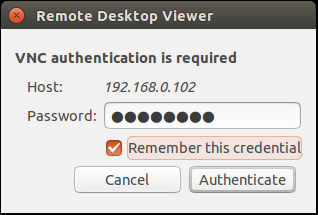
\includegraphics[scale=.45]{remote/images/VNC-3}
\end{center}
\caption{Nhập passwork xác nhận kết nối VNC}\label{Fig:VNC-3}
\end{figure}
\end{list}
\end{list}
